\documentclass[10pt,a4paper]{article}
\usepackage[english]{babel}
\usepackage{multicol}
\usepackage{multirow}
\usepackage{url,hyperref,graphicx,float,times}
\usepackage{sectsty}
\usepackage{authblk}

\renewcommand{\refname}{}

\setlength{\paperheight}{297mm}
\setlength{\paperwidth}{210mm}
\setlength{\voffset}{-12mm}
\setlength{\topmargin}{0mm}
\setlength{\headsep}{8mm}
\setlength{\headheight}{10mm}
\setlength{\textheight}{235mm}
\setlength{\hoffset}{-4mm}
\setlength{\textwidth}{166mm}
\setlength{\oddsidemargin}{0mm}
\setlength{\evensidemargin}{0mm}
\setlength{\marginparwidth}{0mm}
\setlength{\marginparpush}{0mm}
\setlength{\columnsep}{6mm}
\setlength{\parindent}{6mm}
\setlength{\parskip}{2mm}

%% insert eps pictures
%% use as \epsin{epsfile}{width_in_mm}{label}{caption}
\usepackage{epsfig}
\newcounter{figcounter}
\def\epsin #1#2#3#4{
\refstepcounter{figcounter} \label{#3}
\[
\mbox{
  \epsfxsize=#2mm
  \epsffile{#1.eps}
}
\]
%\vspace{0mm}
\begin{center}
  \parbox{7cm}{{\bf FIGURE \arabic{figcounter}:}\quad {\it #4 } } \\
\end{center}
}

%% insert table
%% use as \tabin{size_in_mm}{label}{caption}{table_data}
\newcounter{tabcounter}
\def\tabin #1#2#3#4{
\refstepcounter{tabcounter} \label{#2}
\[ \makebox[#1mm][c]{#4} \]
%\vspace{0mm}
\begin{center}
  \parbox{7cm}{{\bf TABLE \arabic{tabcounter}:}\quad {\it #3 } } \\
\end{center}
}

\title{\LARGE
Performance Evaluation of Xenomai 3
}

\author[*]{\large
{\bf Ching-Chun (Jim) Huang}\thanks{jserv@ccns.ncku.edu.tw}}
\author[*]{\large
{\bf Che-Kang Wu}\thanks{an4006048$@$mail.ncku.edu.tw}}
\author[**]{\large
{\bf Chan-Hsiang Lin}\thanks{r04943031$@$ntu.edu.tw}}
\affil[*]{Department of Computer Science and Information Engineering,
\newline
National Cheng Kung University, Taiwan
\newline
No.1, University Road, Tainan City 701, Taiwan (R.O.C.)}
\affil[**]{Department of Electrical and Electronic Engineering,
\newline
National Taiwan University
\newline
No.1, Sec. 4, Roosevelt Road, Taipei, Taiwan (R.O.C.)}
\date{}


\begin{document}

\maketitle

\begin{abstract}
Xenomai 3 is the new architecture of the real-time framework running seamlessly side-by-side Linux as a dual-kernel system like Xenomai 2, or natively over mainline Linux kernels supplemented by the PREEMPT\_RT efforts to meet stricter response time requirements than standard kernel preemption would bring. In this presentation, we will evaluate the performances of Xenomai 3 running with dual-kernel configuration and analyze the various benchmarks for ARM Cortex-A series. Xenomai 3 introduces some optimizations over RTOS API emulation, thread-to-thread communications, and significantly lower overhead with dual-kernel configurations. The comprehensive performance comparisons illustrate the major evolution of Xenomai 3 along with the revised Real-Time Driver Model (RTDM) which provides a unified interface over both PREEMPT\_RT and dual-kernel.

This paper would be a report on performance measurements among upstream Linux real-time enhancements and Xenomai official stable release (both version 2 and 3 series), and and the benchmarks show that the maximum response time to external interrupts of the dual kernel configurations for Xenomai 3 is almost twice as PPREEMPT\_RT, that more predictable handling on multiple incoming interrupts where Xenomai 3 supports both configurations interchangeably.
\end{abstract}

\vspace{10mm}

\begin{multicols}{2}

%%%%%%%%%%%%%%%%%%%%%%%%%%%%%%%%%%%%%%%%%%%%%%%%%%%%%%%%%%%%%%%%%%%%%%
%% SECTION (REQUIRED)
%%%%%%%%%%%%%%%%%%%%%%%%%%%%%%%%%%%%%%%%%%%%%%%%%%%%%%%%%%%%%%%%%%%%%%
\section{Introduction}
Historically speaking, there are two typical approaches to modifying the standard Linux kernel into a real-time kernel. The first uses an extra small real-time executive \cite{rtai} or microkernel \cite{sel4} which runs the para-virtualized Linux kernel as a task. The small real-time executive takes control over the system for real-time processes and is responsible for scheduling real-time tasks, interrupt handling and scheduling Linux. With these changes it is possible to let a real-time task run on the CPU without the Linux kernel being able to interrupt the task. As the Linux kernel is run as a task it is preemptive at any time.

With the second approach, changes are made the Linux kernel in order to be real-time. This include changes as real-time
scheduling and adding preemption to the kernel.

In this section we briefly present the Xenomai real-time framework for Linux, and the Adaptive Domain Environment for Operating System (Adeos) layer, which allows Xenomai and Linux to run on the same hardware platform.

To provide an objective metric, we run processes on the test system, but measure their performance using an external measurement system which runs a C program on bare metal.

\subsection{Adeos layer}

\textit{Adeos} is a resource virtualization layer, allowing multiple entities called \textit{domains}, that can be seen as complete operating systems, to run  simultaneously on the same hardware platform.

Adeos domains can compete with each other for receiving system generated \textit{events}. Those events can be incoming external (or virtually generated) interruptions, Linux system calls invocations, or various kernel-code-related events like context switches. Adeos introduces the \textit{event pipeline}, which can be seen as a chain of domains of decreasing priority. The events are consequently propagated throughout the pipeline, distributed firstly to the utmost priority domain, then distributed to lower priority domains.

In the case of a Xenomai RTOS running with a Linux kernel, the Adeos pipeline and the organization of the domains is depicted in Figure "EventPipeline". In the pipeline,  we can see that Xenomai has the highest priority, so it can handle and manage first the events before passing them to the Linux kernel. The events can also be blocked by the interrupt shield, preserving the real-time framework from latencies due to event management by the Linux kernel. Throughout this mechanism, Xenomai framework can provide real-time guarantees.

\subsection{Xenomai}

Xenomai provides a kernel-based Application Programming Interface (API) for real-time applications. A user-land API is also available, at the cost of longer latencies. Xenomai introduces the concept of \textit{skins}. Skins are source codes emulating proprietary APIs used for porting real-time applications from various RTOSs such as \textit{VxWorks}, \textit{pSOS}, etc. to Xenomai. When designing a Xenomai application from scratch, the \textit{native} Xenomai skin can be used.

All Xenomai skins rely on the \textit{nucleus}, the core of the RTOS, implementing all algorithms for real-time functionalities. Xenomai provides all standard services one can expect to find in a RTOS: task management, multiple scheduling algorithms, IPCs, etc.

\subsection{Time management in Xenomai}
We focused in this project on periodic real-time tasks that make extensive use of timers. A commonly used skeleton for those tasks in Xenomai as follows :

%\vspace{-0.5cm}
\begin{verbatim}
void myRealTimeTask(void *arg) {
  SetPeriodic(myself, period);
  while(1) {
    /* Do something */
    wait_period();
  }
}
\end{verbatim}
%\vspace{-0.5cm}

The \verb+SetPeriodic()+ function creates and starts a timer related to the calling task, with a period (in clock ticks) equals to the specified parameter. The global tick management function notifies the timer each time a clock tick occurs. When reaching wake up time, the timer executes a handler placing the task in the ready state.

\section{Experiment}

\subsection{Purpose}
1. Compare the performance of Xenomai with baseline Linux kernel and PREEMPT\_RT patched kernel
2. Compare the performance of Xenomai-2 and Xenomai-3
\subsection{Environment Setup}

\subsubsection{Hardware}
For the testing platform, we used the BeagleBone Black. BeagleBone Black is an effective embedded platform with ARM Cortex-A8 processor, capable of running Linux and Xenomai (both 2 and 3), consisting of a single processor, a 512 MB memory, 32kB L1 caches and a 256kB L2 cache.  

\subsubsection{Linux Kernel}
We installed a Debian Linux image\cite{debian} on the beaglebone, with hardware-specific linux kernel from\cite{kernel}. Kernel version 3.14.39 were chosen due to it's compatibility with all kernel configurations.
Four distinct kernel configurations are used for the experiment, as summarized in table\ref{table:config}. Kernel are patched using git merge first, and remaining conflicts are resolved manually.

Kernel configuration options are mostly left as default. However, some of the options may have an impact on real-time latencies. These options include all options under CPU Power Management, APM support, and Opportunistic sleep. Additionally, most debug options in Kernel hacking section lead to increased latencies. Those options are turned off before compilation.

\begin{tabular}{|l| p{3cm} |l|}
\hline
Kernel & Patches & source\\ \hline
mainline   & none & n/a \\ \hline
PREEMPT\_RT & patch-3.14.39-rt37 & \cite{p-rt} \\ \hline
Xenomai 2  & ipipe-core-3.14.39-arm-9 + xenomai v2.6.4 (2015-07-13 HEAD) & \cite{p-ipipe} \cite{git-x2.6} \\ \hline
Xenomai 3  & ipipe-core-3.14.39-arm-9 + xenomai v3.0  & \cite{p-ipipe} \cite{git-x3} \\ \hline
\end{tabular}

\subsubsection{Pre-experiment Settings}
We tried to measure the latencies under 2 conditions - IDLE and CPU-STRESSED. In the IDLE experiment, in order to create such test environment, some redundant user processes were eliminated. While in the CPU-STRESSED condition, these process are also killed, and we used the 'stress' command to keep the CPU busy. The command to kill these processes are written in the test script.

  The gravity values is the shortest time the platform needs to deliver an IRQ to a Xenomai interrupt handler,  a RTDM task running in kernel space, or a user-space task. It is used to differentiate timers on the target context they activate, among IRQ(handler), kernel and user threads, anticipating the next timer shot accordingly, so that such context is activated as close as possible to the ideal time. The gravity values can be set in the file \begin{verbatim}/proc/xenomai/latency on Xenomai-2, /proc/xenomai/clock/coreclk
\end{verbatim} on Xenomai-3 with root privilege. Furthermore, Xenomai-3 has an autotune function that runs a series of internal calibration tests for estimating the most appropriate gravity values for its real-time clock timer, retaining the final values.
Because Xenomai-2 doesn't have an autotune function and it has only one gravity value for all the 
coreclocks, we decided to manually tune all the coreclock values in both Xenomai-2 and Xenomai-3 to zero, so that we can later compare the results on the same basis. 

In our experiments, the kernel build were stored in different SD cards. The fact that different external storage devices have different access specs could affect the result. In order to eliminate the uncertainties, and for the sake of preventing the test process's pages being swapped into disk, we locked all the test process's pages inside memory. In cyclictest, this achieved by specifying the '-m' option in the command. On the other hand, latency is already executed in a memory locked condition.

\subsection{Testing Process}

\subsubsection{Scenario}
The goal of the experiment is to evaluate the realtime performances of Mainline Linux, PREEMPT\_RT, 
Xenomai-2 and Xenomai-3. Also, we want to find out whether the newly released Xenomai-3.0 has improved in realtime capability, compared to Xenomai-2.6.4, the latest stable version of Xenomai-2.
\subsubsection{Tools}
Cyclictest is a commonly-used latency benchmark. It is compatible with all the kernel setups we use (the recently Xenomai-3.0 release add cyclictest to its testsuite), therefore it's suitable for the purpose of measuring latencies for all setups.
Latency is a test program for the Xenomai test suite. It can measure latencies under 3 modes - user task, kernel task, or timer IRQ. It launches the test procedure in one of the user-specified contexts. In the user mode, the measurement task is handled by the 'latency' function in the program, which periodically waits and fetches the current time when resuming. Latency is then measured by calculating the difference of the actual time elapsed with the predefined period.
\subsubsection{Test Procedure}
Each experiment was run on the same hardware. Each was run for 20 minutes to generate approximately 1,000,000 samples. Test scripts were written to facilitate the experiment process.
\subsubsection{Test Load}
As previously mentioned, we measure latencies under IDLE and CPU-STRESSED conditions. In the CPU-STRESSED condition, we called the "stress" process to exert pressure on the CPU.
\subsection{Experiment Result}
\begin{figure}[H]
\begin{center}
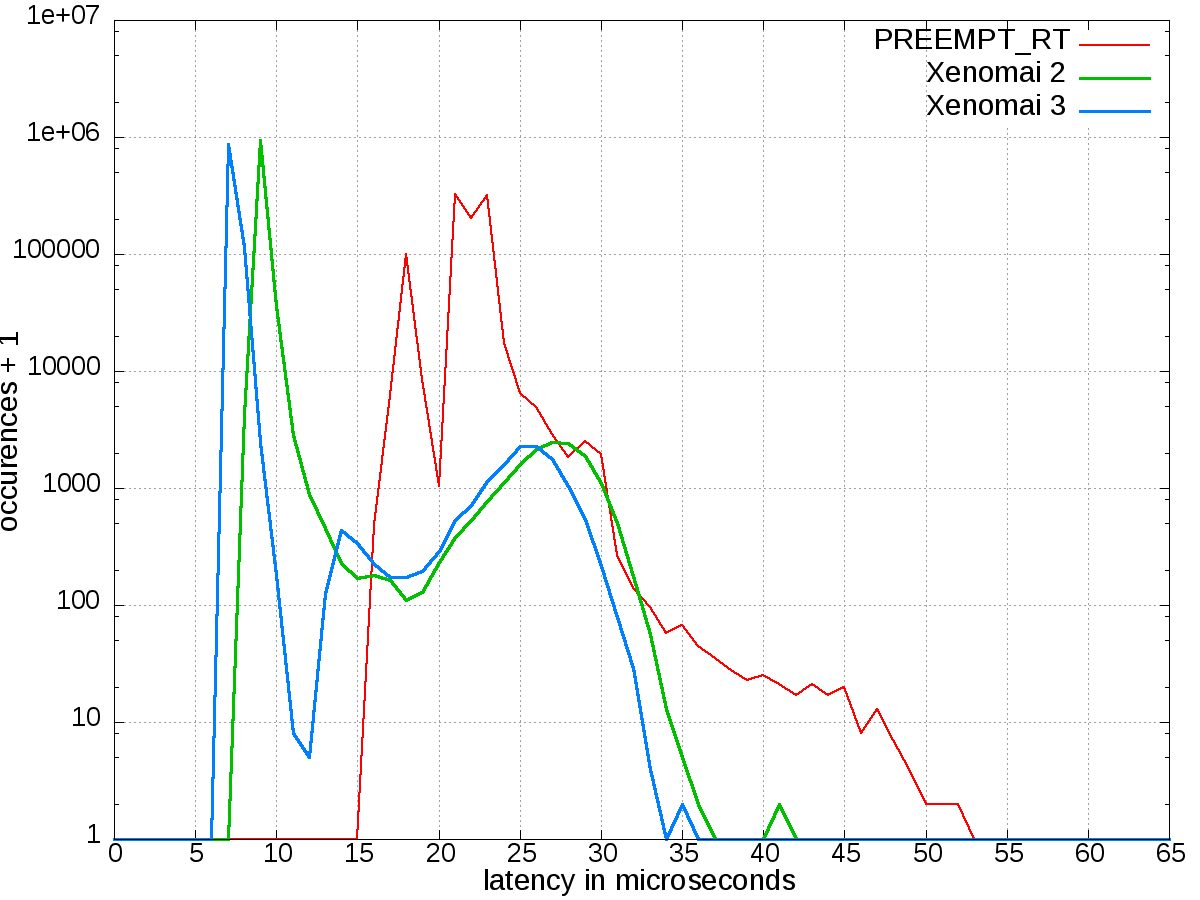
\includegraphics[width=8cm]{img/cyclictest_idle.jpg}
\caption{Cyclictest with no stress.}
\label{cyclictest-idle}
\end{center}
\end{figure}

\begin{figure}[H]
\begin{center}
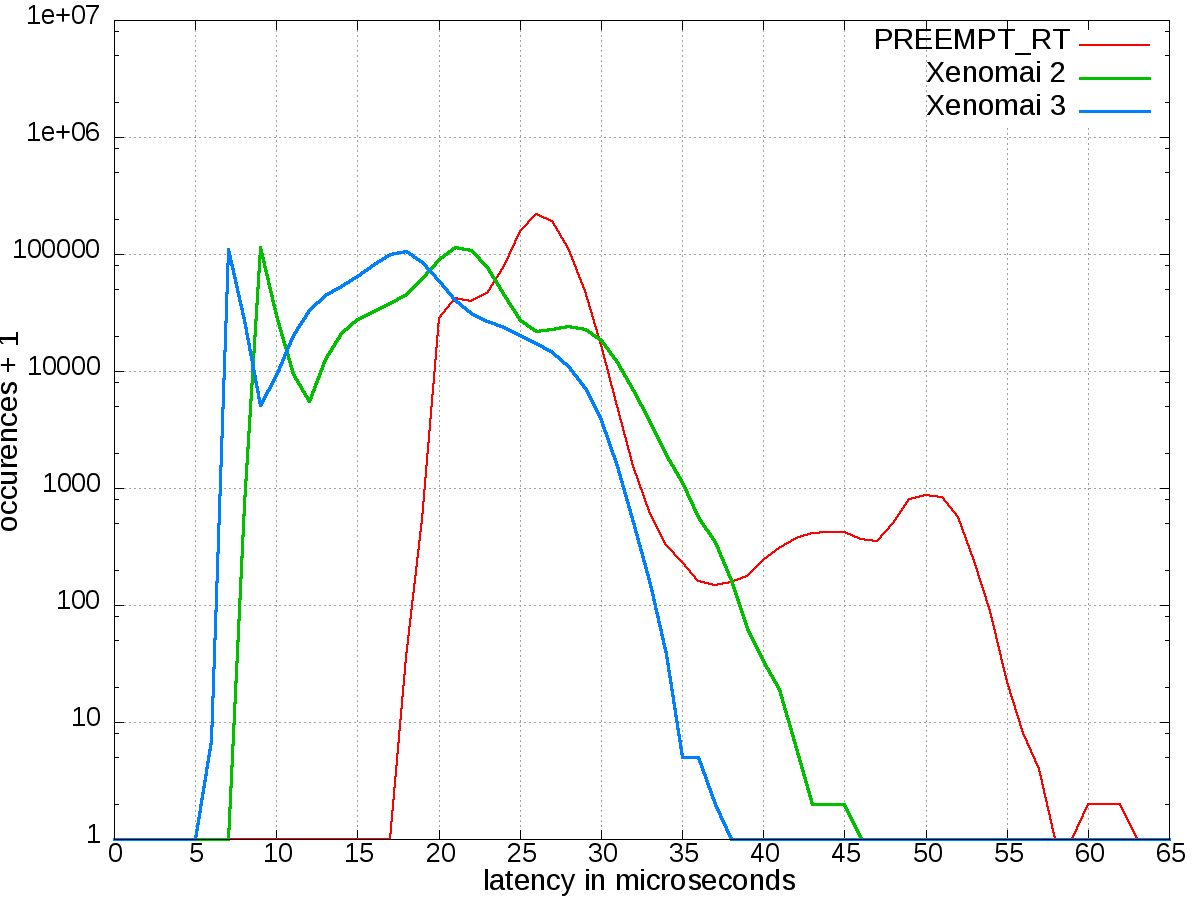
\includegraphics[width=8cm]{img/cyclictest_stress.jpg}
\caption{Cyclictest with stress.}
\label{cyclictest-tress}
\end{center}
\end{figure}

\begin{figure}[H]
\begin{center}
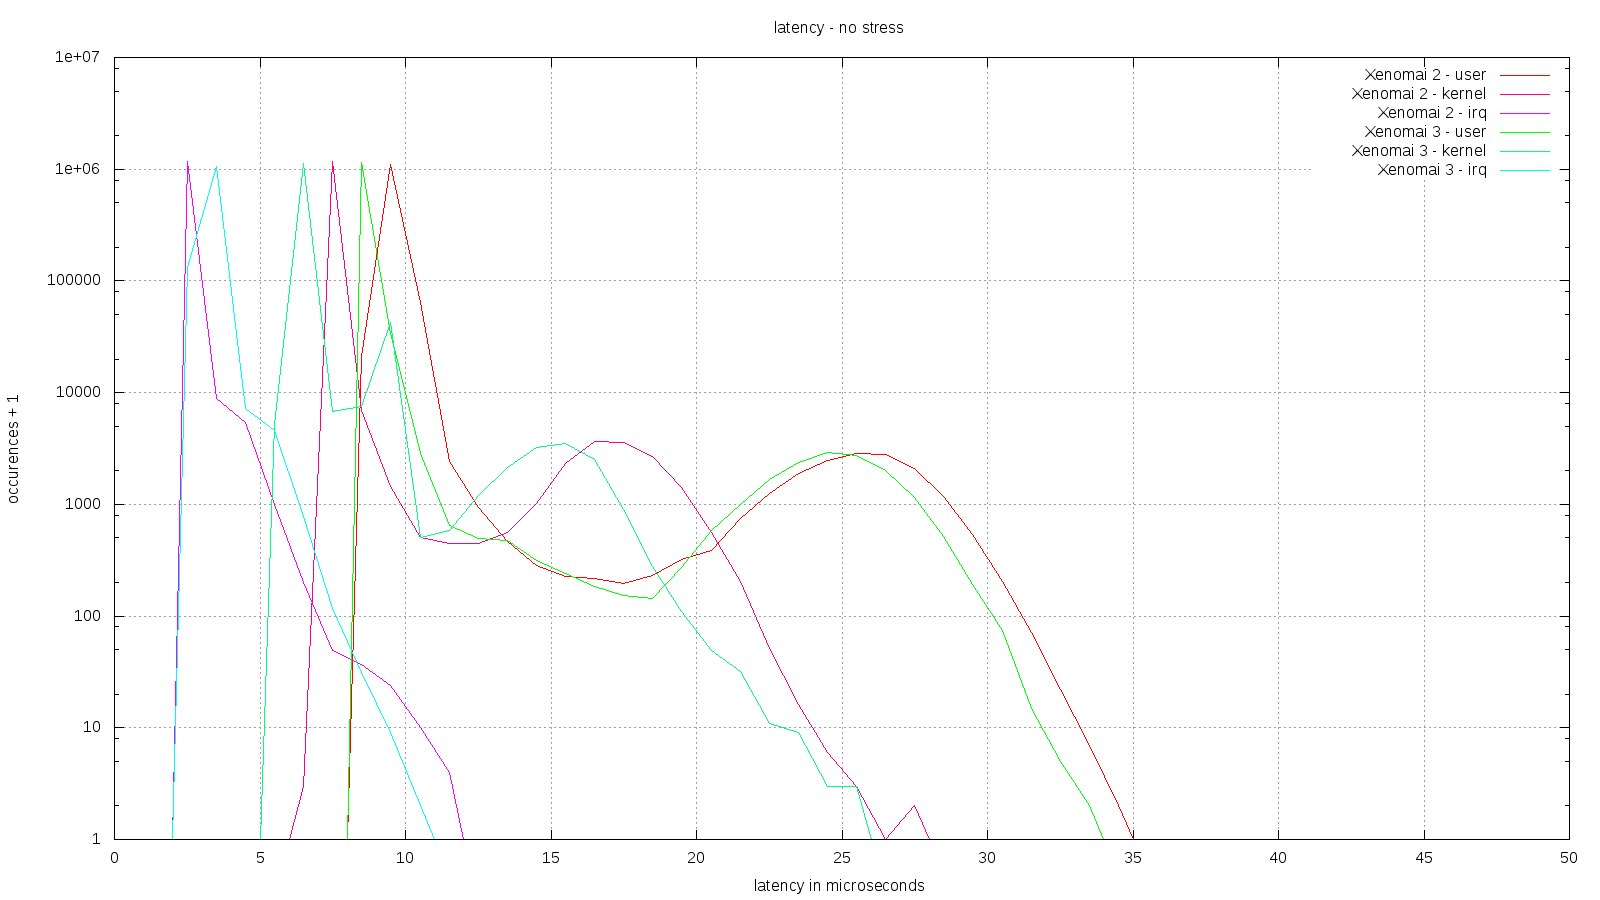
\includegraphics[width=8cm]{img/latency_idle.jpg}
\caption{Latency with no stress.}
\label{latency-idle}
\end{center}
\end{figure}

\begin{figure}[H]
\begin{center}
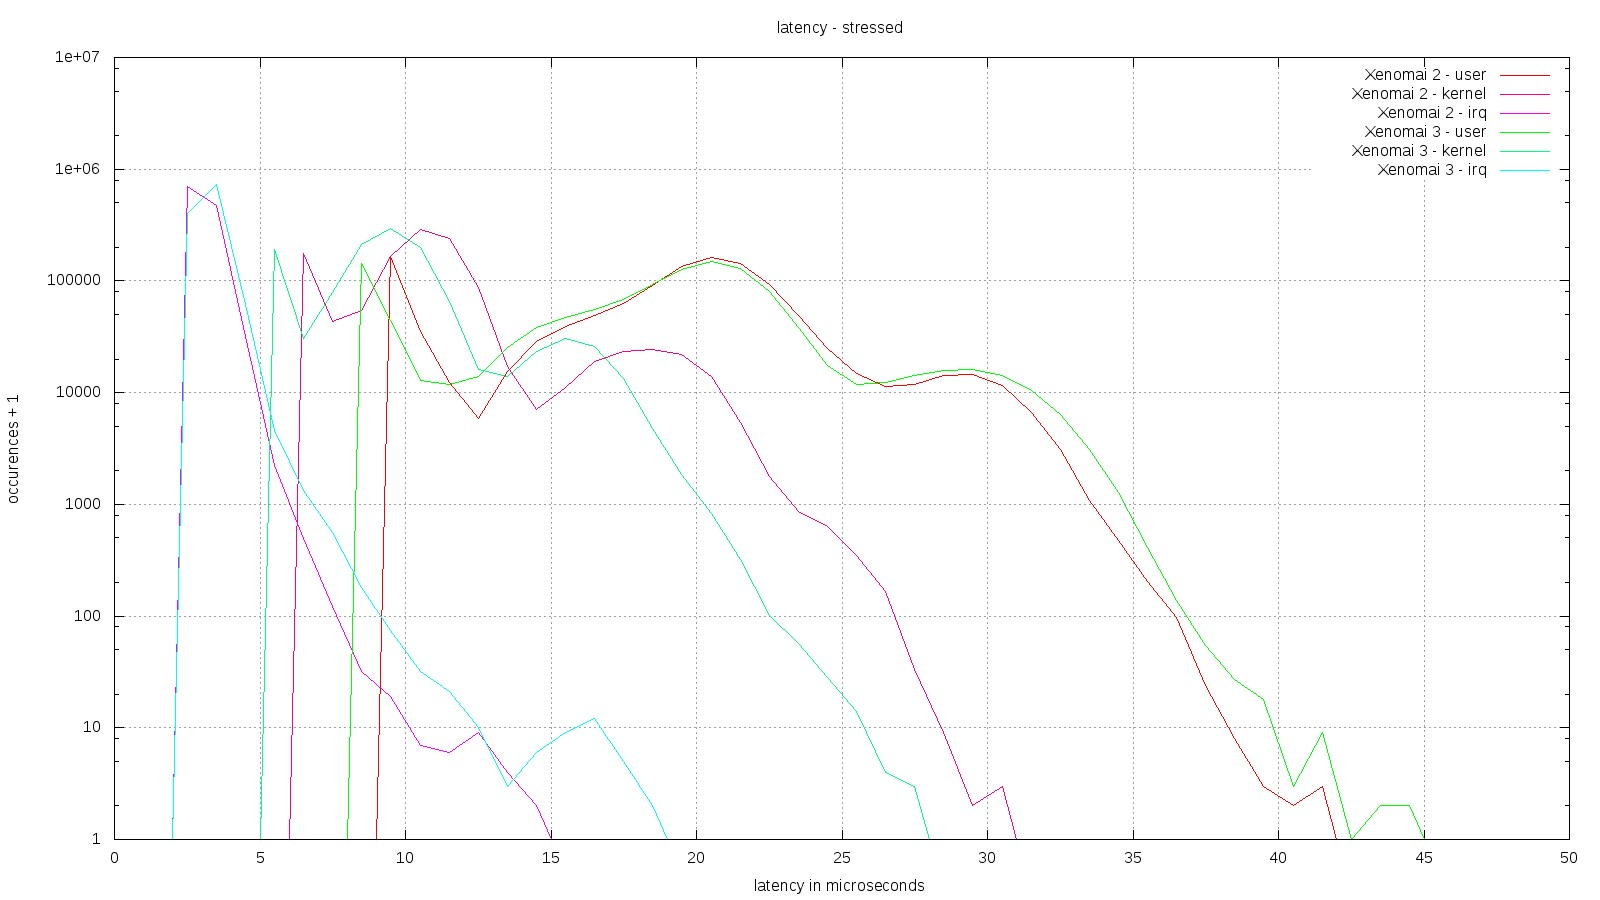
\includegraphics[width=8cm]{img/latency_stress.jpg}
\caption{Latency with no stress.}
\label{latency-stress}
\end{center}
\end{figure}

\epsin{cyclic-idle}{80}{fig2:f2}{Cyclictest Idle}
\epsin{cyclic-cpu}{80}{fig3:f3}{Cyclictest stressed}


\begin{tabular}{|l|c|r|r|}
\hline
\multirow{2}{*}{} & \multicolumn{3}{c|}{user} \\ \cline{2-4} 
 & min & \multicolumn{1}{c|}{avg} & \multicolumn{1}{c|}{max} \\ \hline
Xenomai 2 & 8.541 & 9.458 & 34.583 \\ \hline
Xenomai 3 & 8.043 & 8.853 & 33.023 \\ \hline
& \multicolumn{3}{c|}{kernel}      \\ \hline
Xenomai 2 & 6.965 & 7.708 & 27.821 \\ \hline
Xenomai 3 & 5.567 & 6.479 & 25.577 \\ \hline
& \multicolumn{3}{c|}{timer-irq}   \\ \hline
Xenomai 2 & 2.129 & 2.654 & 11.343 \\ \hline
Xenomai 3 & 2.586 & 3.079 & 10.031 \\ \hline
\end{tabular}


\begin{tabular}{|l|r|r|r|}
\hline
\multirow{2}{*}{} & \multicolumn{3}{c|}{idle}  \\ \cline{2-4} 
 & \multicolumn{1}{l|}{min} & \multicolumn{1}{l|}{avg} & \multicolumn{1}{l|}{max} \\ \hline
Mainline Linux & 39 & 43 & 1046  \\ \hline
Preempt-RT & 16 & 21 & 52 \\ \hline
Xenomai 2 & 8 & 9 & 41 \\ \hline
Xenomai 3 & 7 & 7 & 35 \\ \hline
 & \multicolumn{3}{c|}{cpu-stressed} \\ \hline
Mainline Linux & 39 & 52 & 1097 \\ \hline
Preempt-RT & 18 & 25 & 62 \\ \hline
Xenomai 2 & 8 & 19 & 45 \\ \hline
Xenomai 3 & 6 & 16 & 37 \\ \hline
\end{tabular}


From the data above, it shows that the latency performance of timer-irq in CPU-STRESSED situation is slightly worse on Xenomai-3(over 3 us) than on Xenomai-2(below 3 us). While this is not an occasional case(the same experiment was ran a couple times), we tried to look into the test code of latency to figure out the cause of this phenomenon.

\subsection{Experiment Result Analysis}
Our data shows that the average user-level latency in either Xenomai 2 or 3 is around 9 us in idle situation, 18 us in stressed situation. And in the worse case, the latency is below 50 us. Meanwhile, the latency of PREEMPT\_RT has a user-level latency more than 20 us and can't guarantee a 50 us max latency (Actually in some cases the latency will exceed 100 us in stressed condition).  As for mainline Linux, the max latency easily exceeds 1 ms. When comparing the performance of Xenomai-3 to Xenomai-2, we can see that the stats in cyclictest and latency test is slightly better, except for the case of timer-irq latency in stressed condition.

\section{Conclusions}
The trait of real time in RTLinux is closely related to hardware, So we can take full advantage of PC. The testing on our recorder showed that the average of interrupt response time is 10us, and the max  is 15us. This performance can satisfy this real time requirement of recorder completely and guarantee data integrity. With the high-performance and  great capacity hard disk using, the capacity of the RAID would reach over 1000GB, moreover, collected data don't loss even if one hard disk is demaged.

We had done the test that  under the same hard platform, the recording speed has significantly enhanced in RTLinux than in Windows NT. RTLinux is free, open source, retractile, and transferable, so many OS can not bear comparison with it. RTLinux has been applied successful in our pre-demodulation Digital Recorder; moreover, it will be more widely used in the field of real-time control.

\bibliographystyle{plain}
\begin{thebibliography}{9}%use this if you have <=9 bib refs
	\bibitem {rtai}{\it https://www.rtai.org/}
	\bibitem {sel4}{\it http://ssrg.nicta.com.au/projects/seL4/}
	\bibitem {debian}{\it http://debian.beagleboard.org/images/bone-debian-7.5-2014-05-14-2gb.img.xz}
	\bibitem {kernel}{\it https://github.com/beagleboard/linux}
	\bibitem {p-rt}{\it https://www.kernel.org/pub/linux/kernel/projects/rt/3.14/}
	\bibitem {p-ipipe}{\it http://download.gna.org/adeos/patches/v3.x/arm/ipipe-core-3.14.39-arm-9.patch}
	\bibitem {git-x2.6}{\it http://git.xenomai.org/xenomai-2.6.git/}
	\bibitem {git-x3}{\it http://git.xenomai.org/xenomai-3.git/}
\end{thebibliography}

\end{multicols}
\end{document}
